\documentclass[12pt]{article}
\usepackage[cp1251]{inputenc}
\usepackage[T2A]{fontenc}
\usepackage[english]{babel}
\usepackage{color,graphics}
\usepackage{multirow}
\usepackage{amsmath,amsfonts,amssymb,dsfont}
%\numberwithin{equation}{section}
%\numberwithin{figure}{section}
\usepackage{geometry} 
\geometry{a4paper,top=2cm,bottom=4cm,left=3cm,right=3cm}
\newcommand{\RED}[1]{\textcolor{red}{#1}}
\newcommand{\CYAN}[1]{\textcolor{cyan}{#1}}
\renewcommand{\abstractname}{Abstract}
\renewcommand{\baselinestretch}{1.5}
\everymath{\displaystyle}
\begin{document}
\begin{center}
\noindent{\Large \bf Finite-time thermodynamics: The maximal productivity of binary distillation and selection of optimal separation sequence for an ideal ternary mixture} 
\end{center}

%\vspace*{0.2cm}
\begin{center}
\hspace{0.5cm} \large{A.M. Tsirlin, I.A. Sukin}
\end{center}

\begin{center}
Program Systems Institute RAS, Pereslavl-Zalessky\\
tsirlin@sarc.botik.ru
\end{center}
%\maketitle 

\begin{abstract} 
The paper shows that an attainability region of a binary fractionating column depends on two parameters. These parameters are expressed through kinetic coefficients and mixture properties. The paper also considers a problem of finding the maximal productivity of the ternary distillation. Selection conditions for an optimal separation order and expressions for the maximal productivity of this process were obtained. 
\end{abstract}


\section{Introduction}
  There are many books on the topic of mixture distillation (\cite{Holland}, \cite{Gelp}, \cite{stich}, \cite{shinskey}, \cite{rose}, etc.). The book (\cite{Gelp}, p.540) says that computation methods ``are based on phase equilibrium diagrams and conditions of the material balance, but ignores the kinetics and hydrodynamic properties of apparata. There are some coefficients for filling this gap. These coefficients cannot be computed analytically and must be obtained by approximations or from practice''

We must make an addition to this Gelperin quote. One of the most important things in the column model computation is the irreversibility of the heat transfer process in the reflux drum and the reboiler of the column.
  
  Also, there were only some heuristics for choosing an optimal order of multicomponent mixture separation, for example ``At first one must separate the most easily volatile component'' or ``At first one must separate the component with the largest concentration''. 
  
  Considering the problem of choosing the optimal separation sequence, such estimates are not applicable, because the reversible separation work depends only on the composition of the incoming and outgoing flows. The separation sequence must depend on the irreversible heat consumption.     

     The irreversibility of the mixture separation process is considered in \cite{Berry}, \cite{TsGrig}. Authors there take a look at heat and mass transfer kinetics and its contribution to maximal productivity of the column. However, these papers gives us only an algorithm, but not an analytical relation between these parameters. In this paper such a relation is obtained and applied to an optimal separation sequence selection procedure.
     
     We will use an upper bound of column capabilities, so any of our assumptions must not increase the irreversibility of in-column processes. In this case we can claim that real values do not exceed those we obtained.
     
     First we will write relations defining the boundary of the variety of attainable modes for binary distillation and show that this boundary can be parameterized by a quadratic function. Parametrization coefficients --- (\textit{characteristic coefficients}) --- can be expressed through mixture composition and kinetics constants. Then we will use obtained relations for choosing an optimal separation order of a ternary mixture distillation process.

\section{Limiting capabilities of a binary distillation process}

\begin{figure}[bth]
\centering
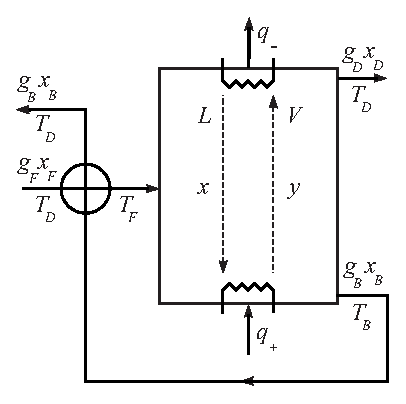
\includegraphics{pic1new1.eps}
\caption{Packed fractionating column and corresponding flows}
\label{fig:pic1new}
\end{figure}

Let us consider a traditional packed fractionating column (Figure \ref{fig:pic1new}) with a reboiler and a reflux drum and using the following assumptions:

1.	Mass transfer is equimolar.

2.	Pressures and temperatures of the vapour and liquid are equal on every horizontal cut (equivalent tray) of the column, but they may vary from one cut to another.

3.	Diffusion effects between adjacent cuts are negligible. 

4.      The heat of the outgoing flows is transmitted to the incoming flows and irreversibility  of heat transfer in this case can be neglected.

5.      The mixture flow is fed in liquid form at boiling into a column cut where the reflux composition is equal to that of the mixture.

   So we consider a model of a packed distillation column with two irreversibility sources: heat transfer in the reboiler and reflux drum and mass transfer in the column itself. The mass transfer coefficient indirectly takes the internal diffusion into account.   

   The molar fractions of the lower boiling component in the feed $x_{F}$ and flows in the reboiler and the reflux drum $x_{B}$ and $x_{D}$ are given. The temperatures in the reboiler ($T_B$) and the reflux drum ($T_D$), determined by evaporation temperatures, are given too. The fraction of the condensate taken from the reflux drum $\varepsilon$ depends on the composition of the outgoing and incoming flows. From material balance of the lower boiling component

\begin{equation}\label{2}
\varepsilon=\frac{x_F-x_B}{x_D-x_B}.
\end{equation}

Assuming the liquid phase is almost an ideal liquid and the vapour phase is almost an ideal gas,  equilibrium concentrations of the lower boiling component in vapour and liquid have this relation
\begin{equation}\label{5.42}
y^0(x)= \frac{\alpha x}{1+(\alpha-1)x},
\end{equation}
where  $y$ --- lower boiling component concentration in the vapour, $\alpha= \frac{P_1^0(T)}{P_2^0(T)}>1$ --- relative volatility coefficient, $P_i^0$ --- pressure of a saturated vapour above the pure $i$-th component ($i$=1 for lower boiling one). 

We will not consider peculiarities of azeotropes, but our approach can be applied to mono-azeotropes if one uses a mixture with a composition corresponding to the azeotropic point as a quasi-component.

\vspace*{0.3cm}
\textbf{Thermodynamical balances of a binary distillation and the relation between the heat consumption and  the productivity of the column.}

Assuming the mixing heat can be neglected, energy and entropy balances are 

\begin{equation}\label{5.44}
q_{+} - q_{-} + g_{F} h_{F} - g_{F}\varepsilon h_{D} - g_{F}(1-\varepsilon) h_{B} = 0,
\end{equation}
\begin{equation}\label{5.45}
g_{F} s_{F} - g_{F}\varepsilon s_{D} - g_{F}(1-\varepsilon) s_{B}+ \frac{q_{+}}{T_B} -
\frac{q_{-}}{T_D} + \sigma = 0.
\end{equation}
where $\sigma>0$  --- entropy production in the column.
 
 From (\ref{5.44}), (\ref{5.45}) after elimination of $q_{-}$ we will get
\vspace{-0.1cm}
$$\hspace{-3.5cm}
q_{+}= g_{F}\frac{T_B}{T_B- T_D}\Big[(s_{F} T_D-h_{F})- \varepsilon
(s_{D} T_D- h_{D})-
$$
\begin{equation}\label{5.46}
\phantom{aaaaaaaaaa} - (1-\varepsilon) (s_{B} T_D- h_{B})\Big]+ \sigma
\frac{T_B T_D}{T_B- T_D}= q^0_{+}+ \sigma \frac{T_B T_D}{T_B-
T_D}.
\end{equation}
The first summand in the right part of this expression $q^0_{+}$, is the heat consumption in a reversible process, when heat and mass transfer coefficients are arbitrarily large. It depends only on parameters of the outgoing and incoming flows and is proportional to the productivity  $g_F$. The second summand is the irreversible energy losses.

External outgoing and incoming heat flows usually go through heat exchangers where hot flows are cooled down and feed flow is warmed up to the temperature on the feed plate. We will include these heat exchangers in our system considering that irreversible losses in them are negligible. So we can consider that all of external flows have the same temperature approximately equal to $T_D$. In this case $q_+=q_-=q$. 

Considering that the difference $(h-T_D s)$ is the same for any flow and is equal to a free molar energy or a chemical potential  $\mu$  of the mixture at $T=T_D$,  we can get a relation between heat flow and the productivity in the following form
\begin{equation}\label{46m}
q= g_{F}\frac{T_B}{T_B- T_D}\Big[ \varepsilon \mu(T_D,x_D)+(1-\varepsilon)\mu(T_D,x_B)   
-\mu(T_D,x_F)\Big]+ \sigma \frac{T_B T_D}{T_B-
T_D}.
\end{equation}

Every chemical potential expression looks like
\begin{equation}\label{5.61}
\mu_i(T, P, x_i)= \mu_{i0}(P, T)+ RT \ln x_i,\quad i=D,B,F.
\end{equation}

Because chemical potentials in every individual column cut correspond to the same pressure and temperature their difference for the vapour phase is
$$
\mu_1(T, y^0)- \mu_1(T, y)= RT \ln \frac{y^0}{y},
$$
$$
\mu_2(T, 1-y)- \mu_2(T, 1-y^0)=RT \ln \frac{1-y}{1-y^0}.
$$

The right part of (\ref{46m}) can be expressed through the flow composition
\begin{equation}\label{46n}
q= g_{F}\frac{T_B}{T_B- T_D}\Big[ A_F-\varepsilon A_D-(1-\varepsilon)A_B\Big]+\frac{\sigma T_DT_B}{T_B- T_D}=\frac{p_0}{\eta_{{\mbox{\scriptsize K}}}}+ \frac{\sigma T_D}{\eta_{{\mbox{\scriptsize K}}}}.
\end{equation}
where $ A_i=-RT_D\Big[x_ilnx_i +(1-x_i)ln(1-x_i)\Big](i=F,D,B)$ is the reversible separation work for one mole of $i$-th flow into the pure components. The expression in the square brackets is the reversible Gibbs separation work for one mole of feed flow with concentration $x_F$ to the flows with concentrations $x_D$, $x_B$ at the temperature $T_D$. We will denote it as $A_G$. Value $\eta_{{\mbox{\scriptsize K}}}= (1- {T_D}/{T_B})$ is analogous to the Carnot energy conversion efficiency. Given entropy in (\ref{46n}) is equal to zero, we will get a reversible estimate $q^0=\frac{g_FA_G}{\eta_{{\mbox{\scriptsize K}}}}$ of distillation heat consumption. Reversible rectification looks like an ideal heat engine working between reservoirs with temperatures $T_B$ and $T_D$ and producing the separation power $p^0=g_F A_G$.

Solving  equation (\ref{46n}) for $g_F$
\begin{equation}\label{46n1}
g_F=q\frac{\eta_{{\mbox{\scriptsize K}}}}{A_G}-\sigma(q,g_F)\frac{T_D}{A_G}.
\end{equation}
Let us find a lower bound of the second summand in this expression.
 

\vspace*{0.3cm}
\textbf{Irreversible energy losses}

\textit{Heat transfer irreversibility}. Assuming the heat flows in the reboiler and the reflux drum are proportional to the temperature difference,
\begin{equation} 
q=rV=\beta_{B}(T_+-T_B)=\beta_{D}(T_D-T_-).
\label{q3a}
\end{equation}
where $V$ --- a flow of the vapour coming from the reboiler, $r$ --- molar vaporization heat.

Entropy production from heat transfer processes in the reboiler and the reflux drum is
\begin{equation}
\sigma_q = q\Big[\frac{1}{T_B}-\frac{1}{T_+}+\frac{1}{T_-}-\frac{1}{T_D} \Big]=q^2\Big[\frac{1}{\beta_{B}T_B T_{+}} +\frac{1}{\beta_{D}T_D T_{-}}\Big],
\label{q3}
\end{equation}
where $\beta_{B}$ and $\beta_{D}$ --- heat transfer coefficients, proportional to the surface of the heat transfer process, $T_B$ and $T_D$ are the given temperatures of the liquid in reboiler and reflux drum. 

Given the heat flow, temperatures $T_+$ and $T_-$ depend on selected reboiler and reflux drum temperature differences. Substituting them into (\ref{q3}) we can get the value of $\sigma_q$.

\textit{Mass transfer irreversibility}. Let us assume that we have a model of the packed fractionating column with the liquid back-flowing relative to the vapour, working in the mode close to the ideal liquid displacement.
 The vapour flow $V=\frac{q}{r}$ given equimolar mass transfer is constant and is related to reflux flow $L$ by the following relations

for the upper part of the column
\begin{equation}
L_{D} = \frac{q}{r}-  g_D,
\label{q1}
\end{equation}

for the lower part of the column
\begin{equation}
L_{B}= \frac{q}{r}+ g_{B}.
\label{q2}
\end{equation}

Given that for binary distillation concentrations of the higher boiling component in the liquid and vapour flows are equal to $1-x$ and $1-y$ respectively, and the driving force of the mass transfer process depends on the difference of the current concentration $y(x)$ and equilibrium concentration $y^0(x)$, we can express the entropy production for mass transfer through flows and chemical potentials as
$$
\sigma_g= \int\limits^{x_D}_{x_B}\frac{1}{T(x)} \{ g_1(y, y^0) [ \mu_1(T, y^0) \;
-\mu_1(T, y)]+\phantom{wwwwwwwwwwwwwwwwwwwwwwww}
$$
\begin{equation}\label{5.60}
+ g_2(1-y, 1-y^0)[ \mu_2(T, 1-y)- \mu_2(T, 1-y^0)] \} \; dx,
\end{equation}
where $g_j$ and $\mu_j$ (j=1,2) are mass flows and chemical potentials of the components.

Expression (\ref{5.60}) can be rewritten with respect to (\ref{5.61}) and ($g_1(y, y^0)=- g_2(1-y, 1-y^0)=g$) as
\begin{equation}\label{5.62}
\sigma_g=R \int\limits^{x_D}_{x_B} g(y, y^0)\ln \frac{y^0(1-y)}{y(1-y^0)} \; dx.
\end{equation}
We assumed that feed flow $g_{F}$ has the liquid form and is fed at its evaporation temperature to the column cut where its composition is equal to the reflux's one, so the entropy production from mixing can be neglected.


The entropy production from mass transfer processes depends on the form of equilibrium and working lines. The first one is determined by the parameters of the given mixture (relative volatility coefficient $\alpha$ (\ref{5.42})), and the second one is determined by $V=\frac{q}{r}$. From the material balance equation for the lower boiling component we can get, for the upper and lower parts of the column
\begin{equation}
\frac{q}{r}y(x)- g_{D} x_{D} - x L_{D} =0,
\label{q4}
\end{equation}
\begin{equation}
L_{B} x - \frac{q}{r}y (x)- g_{B} x_{B} =0.
\label{q5}
\end{equation}
Given (\ref{q1}), (\ref{q2}) after substitution $g_D=g_F\varepsilon$, $g_B=g_F(1-\varepsilon)$ working lines will be in the form
\begin{equation}
y^{D} (x, \frac{q}{r}, g_F)= \left( 1- \frac{g_F\varepsilon r}{q} \right) x + \frac{x_{D}
g_F\varepsilon r}{q},
\label{q6}
\end{equation}
\begin{equation}
y^{B} (x, \frac{q}{r}, g_{F})= \left( 1+ \frac{g_F(1-\varepsilon)r}{q} \right) x - \frac{x_{B}
g_F(1-\varepsilon)r}{q}
\label{q7}
\end{equation}
which leads us to $y^{D}(x_D)=x_D,~y^{B}(x_B)=x_B,\quad y^{D}(x_F)= y^{B}(x_F)=y_F$, and $y_F-x_F=\frac{g_D r}{q}(x_D-x_F)$.

Substituting (\ref{q6}), (\ref{q7}) into (\ref{5.62}) gives the value of $\sigma_g (q, g_{F})$ for the given mass transfer law. The integral value must be computed as the sum of integrals over intervals from $x_{B}$ to $x_{F}$, where $y(x)=
y^{B} (x, \frac{q}{r},g_F)$, and from $x_{F}$ to $x_{D}$, where $y(x)= y^{D} (x, \frac{q}{r},g_F)$. That operation can be performed only numerically.

Let us find the lower estimate of $\sigma_g$, assuming that mass transfer  is proportional to the driving force,
\begin{equation}
g(y, y^0)= k\frac{[ \mu_1(T, y^0)-\mu_1(T, y)]}{T}.
	\label{r8}
\end{equation}
After eliminating the chemical potential difference through introducing flow values $g(y, y^0)$, equation (\ref{5.62}) takes the form
\begin{equation}
\sigma_g (q,g_F)=\frac{2}{k}\int\limits^{x_D}_{x_B} g^2(y, y^0)dx .
	\label{r4}
\end{equation}
The factor of 2 comes from the higher boiling component flow's equimolarity.

Given the following flow average value
\begin{equation}
\bar{g}=\frac{1}{x_D-x_B}\int\limits^{x_D}_{x_B} g(y, y^0)dx
\label{r4a}
\end{equation}
and using (\ref{r4}) we can find the lower estimate of $\sigma_g$. The following is true, indeed
\begin{equation}
\int\limits^{x_D}_{x_B} [g(y, y^0)-\bar{g}]^2 dx=\frac{k\sigma_g}{2}+(x_D-x_B)\bar{g}^2-2\bar{g}\int\limits^{x_D}_{x_B} g(y, y^0)dx.
\label{r4b}
\end{equation}
The left hand side of this equation is non-negative and the third summand of the right hand side is equal to twice the second one. Solving (\ref{r4b}) for $\sigma_g$, we will get our estimate in the form
\begin{equation}
\sigma_g\geq\frac{2(x_D-x_B)\bar{g}^2}{k}.
\label{r4c}
\end{equation}
The inequality becomes an equality if mass transfer flow weakly depends on the current individual column cut.

Since vapour consumption at the top of the column is constant, we can write the following material balance condition 
\begin{equation}
\int\limits^{x_{D}}_{x_{B}}\!g(y , y^0 ) dx=V[y^D(x_D)-y^B(x_B)]=\frac{q}{r}(x_D-x_B),
\label{q8}
\end{equation}
the vapour flow is $\bar{g}=\frac{q}{r}$ and
\begin{equation}
\sigma_g\geq\frac{2(x_D-x_B)q^2}{kr^2}.
\label{r4d}
\end{equation}
The right part of this expression will be used for estimating the mass transfer irreversibility. Our task is to get the upper estimate for attainable productivity, so we can assume that (\ref{r4d}) is an equality.

\subsection {Relation between the column's productivity and the heat consumptive given irreversibility}
Substituting the total entropy production $\sigma = \sigma_q + \sigma_g$ into (\ref{46n1}) we can get an estimate of the binary distillation productivity
\begin{equation}
g_F= bq-aq^2, 
\label{w4e}
\end{equation} 
where the characteristic coefficients $a$ and $b$ depend on the processes kinetics and mixture composition as
 \begin{equation}
 a=\Big[\frac{1}{\beta_{B}T_B T_{+}} +\frac{1}{\beta_{D}T_D T_{-}}+\frac{2(x_D-x_B)}{kr^2}\Big]\frac{T_D}{A_G},
\label{r4e}
\end{equation} 
\begin{equation}
 b=\frac{T_B - T_D}{T_B A_G}=\frac{\eta_k}{A_G}.
\label{b4e}
\end{equation} 

We must note that the form of the boundary of binary distillation column attainable modes depends only on two parameters, each is determined by mixture parameters and column mode. The first parameter $b$ is called the \textit{reversible efficiency coefficient}, and the second one $a$ is called the \textit{irreversibility coefficient}. The reversible efficiency coefficient depends only on the composition of the mixture flows whereas the irreversibility coefficient depends also on processes kinetics.

The maximal heat consumption and the maximal productivity determined by the characteristic coefficients. The productivity is maximal at
\begin{equation}\label{46n4}
q^0=\frac{b}{2a}
\end{equation}
and takes the maximal value of
\begin{equation}\label{46n5}
g_F^m=\frac{b^2}{4a}.
\end{equation}

The interval from zero to the heat flow value $q^0$ forms the useful area of the column attainable modes. Further heat flow increase leads only to productivity decreasing.

You can easily see that column efficiency value, given irreversibility, $\eta=\frac{g_F}{q}$ for the mode with the maximal productivity doesn't depend on irreversible parameters and is equal to $0,5b$ (the half or the reversible efficiency coefficient). This corresponds to the fact that the efficiency (Novikov-Curzon-Ahlborn efficiency) of an irreversible heat engine for its maximal power cycle doesn't depend on heat transfer kinetics, but maximal power itself does. 

The effective mass transfer coefficient $k$ in (\ref{r4e}) is assumed to be given. There is a description of the method for calculating this coefficient in the Appendix.

The heating vapour temperature $T_+$ is slightly higher than the temperature in the reboiler $T_B$, and the cooling water temperature $T_-$ is slightly lower than $T_D$. They can be expressed through heat flow and heat transfer coefficients but for getting estimates we can assume these temperatures to be equal to $T_B$ and $T_D$ respectively, neglecting the difference of 7--15 degrees.

 
\section {Ternary mixture. The variety of attainable modes and selection of optimal separation sequence.}
Some problems can be solved using (\ref{r4e}), (\ref{b4e}).

The distillation process is highly power-consuming so it is sensibly to choose the separation order so it will minimize the heat consumption for the given productivity and flow composition. For simplicity we will assume that distillation in each column is complete, e.g. the mixture is separated into pure components.

Mixture components must be arranged so that the evaporation temperature is maximal for the component with a concentration $x_2$. We will introduce the notation for characteristic coefficients of each distillation order:

--- Direct order (Fig. \ref{fig:direct}), when the first column separates the component with zero index and the second column separates components with indices one and two. Corresponding characteristic coefficients will have the index 1. For example, $b_{11}$ is the reversible efficiency coefficient of the direct distillation order for the first column.

--- Indirect order (Fig. \ref{fig:indirect}), when the first column separates the component with the index two and the second column separates two other components. So $b_{21}$ is the reversible efficiency coefficient of the indirect distillation order for the first column.

\begin{figure}[bth]
\centering
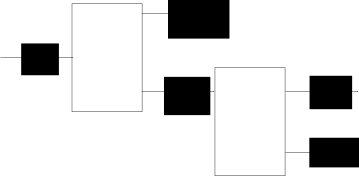
\includegraphics{direct.eps}
\caption{Direct distillation order. A, B and C are the mixture components.}
\label{fig:direct}
\end{figure}

\begin{figure}[bth]
\centering

\includegraphics{indirect.eps}
\caption{Indirect distillation order. A, B and C are the mixture components.}
\label{fig:indirect}
\end{figure}

At first we must find the values of  $a_{ij}, b_{ij},i=1, 2;\quad j=1, 2$ using (\ref{r4e}), (\ref{b4e}).

Given a mixture with the concentrations $x_0$, $x_1$, $x_2$, we will assume that $x_0$ is the lower boiling component concentration and $x_2$ is the higher boiling component concentration. Also, we will assume that relative volatilities $\alpha_{01}$ and $\alpha_{12}$ are known, as are molar vaporization heats of lower boiling $r_0$ and middle boiling $r_1$ components. Molar vaporization heat of the mixture of lower boiling and middle boiling components is the weighted average $r_{01} = (r_0x_0 + r_1x_1)/(x_0+x_1)$. Corresponding evaporation temperatures will be denoted as $T_0$, $T_1$ and $T_2$.

In the case of the direct distillation order:
\begin{itemize}
\item Mass transfer coefficient for the first column $k_{11}$;
\item Mass transfer coefficient for the second column $k_{12}$;
\item Heat transfer coefficients for the first column in the reboiler and reflux drum respectively $\beta^B_{11}$, $\beta^D_{11}$;
\item Heat transfer coefficients for the second column $\beta^B_{12}$, $\beta^D_{12}$;
\end{itemize}

Characteristic parameters in this case can be calculated as, for the first column:
\begin{equation}
b_{11} = -\frac{T_1 - T_0}{RT_0T_1\left[x_0\ln{x_0} + (1-x_0)\ln{(1-x_0)}\right]},
\label{eq:b1c1v}
\end{equation}
\begin{equation}
a_{11} = -\left[\frac{1}{\beta^B_{11}T_1^2} + \frac{1}{\beta^D_{11}T_0^2} + \frac{2}{k_{11}r_0^2}\right]\frac{1}{R\left[x_0\ln{x_0} + (1-x_0)\ln{(1-x_0)}\right]}.
\label{eq:a1c1v}
\end{equation}
For the second column:
\begin{equation}
b_{12} = -\frac{T_2 - T_1}{RT_1T_2(\frac{x_1}{1-x_0}\ln{\frac{x_1}{1-x_0}} + \frac{x_2}{1-x_0}\ln{\frac{x_2}{1-x_0}})},
\label{eq:b2c1v}
\end{equation}
\begin{equation}
a_{12} = -\left[\frac{1}{\beta^B_{12}T_2^2} + \frac{1}{\beta^D_{12}T_1^2} + \frac{2}{k_{12}r_1^2}\right]\frac{1}{R(\frac{x_1}{1-x_0}\ln{\frac{x_1}{1-x_0}} + \frac{x_2}{1-x_0}\ln{\frac{x_2}{1-x_0}})}.
\label{eq:a2c1v}
\end{equation}

For the indirect distillation order:
\begin{itemize}
\item Mass transfer coefficient for the first column $k_{21}$;
\item Mass transfer coefficient for the second column $k_{22}$;
\item Heat transfer coefficients for the first column $\beta^B_{21}$, $\beta^D_{21}$;
\item Heat transfer coefficients for the second column $\beta^B_{22}$, $\beta^D_{22}$;
\end{itemize}

Characteristic coefficients in this case can be calculated as, for the first column:
\begin{equation}
b_{21} = -\frac{T_2 - T_1}{RT_2T_1\left[(x_0+x_1)\ln{(x_0+x_1)} + x_2\ln{x_2}\right]},
\label{eq:b1c2v}
\end{equation}
\begin{equation}
a_{21} = -\left[\frac{1}{\beta^B_{21}T_2^2} + \frac{1}{\beta^D_{21}T_1^2} + \frac{2}{k_{21}r_{01}^2}\right]\frac{1}{R\left[(x_0+x_1)\ln{(x_0+x_1)} + x_2\ln{x_2}\right]}.
\label{eq:a1c2v}
\end{equation}
For the second column:
\begin{equation}
b_{22} = -\frac{T_1 - T_0}{RT_1T_0(\frac{x_0}{1-x_2}\ln{\frac{x_0}{1-x_2}} + \frac{x_1}{1-x_2}\ln{\frac{x_1}{1-x_2}})},
\label{eq:b2c2v}
\end{equation}
\begin{equation}
a_{22} = -\left[\frac{1}{\beta^B_{22}T_1^2} + \frac{1}{\beta^D_{22}T_0^2} + \frac{2}{k_{22}r_0^2}\right]\frac{1}{R(\frac{x_0}{1-x_2}\ln{\frac{x_0}{1-x_2}} + \frac{x_1}{1-x_2}\ln{\frac{x_1}{1-x_2}})}.
\label{eq:a2c2v}
\end{equation}

We must analyze the relation between the cascade productivity and the heat consumption given parameterized representation for each distillation order.

The maximal productivity of the cascade is equal to the one of the first column (because the maximal productivity of the second column is limited by the outgoing flow from the first one): 
\begin{equation}
g_F^* = \frac{b_{i1}^2}{4a_{i1}}.
\label{eq:max-perf}
\end{equation}
As the first column one should take the column with the greater maximal productivity, because the reversible efficiency coefficient does not depend on kinetics.

\textbf {Consistency conditions.}
The columns must be coordinated in such a way that the maximal productivity of the first column must match the allowed productivity of the second column by the incoming two-component flow. This leads to the following inequalities:

--- for the direct distillation order
\begin{equation}
\frac{b_{12}^2}{(1-x_0)a_{12}} \geq \frac{b_{11}^2}{a_{11}},
\label{eq:s1}
\end{equation}


--- for the indirect distillation order
\begin{equation}
\frac{b_{22}^2}{(1-x_2)a_{22}} \geq \frac{b_{21}^2}{a_{21}}.
\label{eq:s2}
\end{equation}

Since the maximal productivity increase requires increasing the column size (or heat transfer surfaces), in the optimal case the maximal productivity of the second column by the incoming two-component flow must be equal to the maximal productivity of the first column. In this case inequalities (\ref{eq:s1}), (\ref{eq:s2}) become equalities and are called \textit{full consistency conditions}.

Given the full consistency conditions:
\begin{equation}
a_{12} = a_{11}\frac{b_{12}^2}{b_{11}^2(1-x_0)},\quad a_{22} = a_{21}\frac{b_{21}^2}{b_{22}^2(1-x_2)}.
\label{eq:s3}
\end{equation}

\paragraph{Calculating the maximal heat consumption. Attainability boundary of the column cascade.}

We will write our equations for the direct distillation order. The indirect order can be treated in a similar way. 

Considering the cascade of two columns with productivities:
\begin{equation}
g_F = b_{11} q_1
\end{equation}
and
\begin{equation}
g_F(1-x_0) = b_{12} q_2,
\end{equation}
we will get the reversible estimate for the cascade productivity depending on the total heat flow $q$,
\begin{equation}
g_F = \frac{b_{11}b_{12}(q_1+q_2)}{b_{12}+b_{11}(1-x_0)}.
\label{eq:casc-r}
\end{equation}
The reversible efficiency coefficient of the cascade is
\begin{equation}
b^I = \frac{b_{11}b_{12}}{b_{12}+b_{11}(1-x_0)}
\label{eq:b-casc}
\end{equation}
for the direct order and
\begin{equation}
b^{II} = \frac{b_{21}b_{22}}{b_{22}+b_{21}(1-x_2)}
\label{eq:b-casc2}
\end{equation}
for the indirect order.

If every incoming flow is much smaller than the maximal productivity, the distillation order is determined by comparison of relative effectiveness coefficients. On lower loads the direct order is preferred because $b_{ij}$ depends on the composition of the feed when
\begin{equation}
\frac{b_{11}b_{12}}{b_{12}+b_{11}(1-x_0)}>\frac{b_{21}b_{22}}{b_{22}+b_{21}(1-x_2)}.
\label{eq:b1-casc2}
\end{equation}
Through properties of the feed (\ref{eq:b1-casc2}) can be rewritten as
\begin{equation}
T_2(T_1 - T_0) > T_2(T_1 - T_0).
\label{eq:b1-sc2}
\end{equation}

\begin{figure}[bth]
\centering
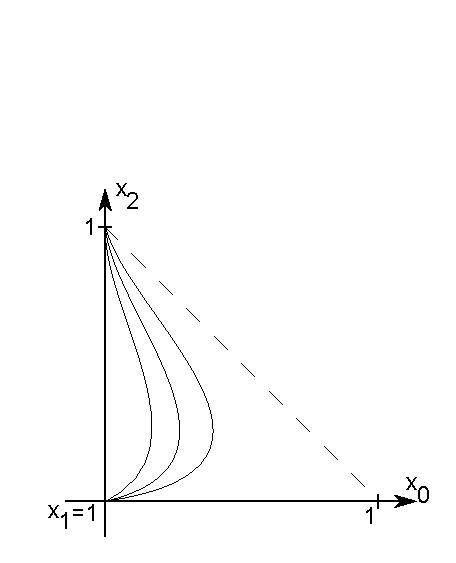
\includegraphics{simplex.eps}
\caption{Regions of the concentration simplex in the $(x_0,x_2)$ plane with different preferred order, considering irreversibility. Direct order is preferred ``to the right'' of the curves. Different curves correspond to different values of given $g_F$.}
\label{fig:pic5}
\end{figure}

In the general case one must consider irreversibility issues. Given the following attainability region boundaries for the $i$-th distillation order,
\begin{equation}
g_F = b_{i1} q_{i1} - a_{i1} q_{i1}^2
\label{eq:1c}
\end{equation}
and
\begin{equation}
g_F (1-x^i) = b_{i2} q_2 - a_{i2} q_{i2}^2.
\label{eq:2c}
\end{equation}

Expressing $q_{i1}$ and $q_{i2}$ from (\ref{eq:1c}), (\ref{eq:2c}) through $g_F$ gives
\begin{equation}
q_{i1} = \frac{b_{i1} - \sqrt{b_{i1}^2 - 4a_{i1}g_F}}{2a_{i1}}
\label{eq:1cq}
\end{equation}
and
\begin{equation}
q_{i2}= \frac{b_{i2} - \sqrt{b_{i2}^2 - 4a_{i2}g_F(1-x^i)}}{2a_{i2}}\RED{,}
\label{eq:2cq}
\end{equation}
where $i$ is the distillation order (direct --- $i=1,\quad x^i=x_0$, indirect --- $i=2,\quad x^i=x_2$).
 
For the given productivity and computed values of characteristic coefficients these expressions help us find the heat consumptions for each column and choose the distillation order for which the total consumption is minimal. It's pretty obvious that distillation order depends on the feed composition, evaporation temperatures, molar vaporization heats and kinetics coefficients of heat and mass transfer.

Figure \ref{fig:pic5} shows the division of the concentration simplex (the $(x_0,x_1)$ plane) into areas where one or the other distillation order is preferred. The direct order is preferred in the region above the curve. Curve 2 corresponds to considering irreversibility (\ref{eq:1c}) and curve 1 corresponds to (\ref{eq:b1-sc2}).

Expressions are especially simple when the two columns are fully consistent. Substituting (\ref{eq:s3}) into (\ref{eq:2cq}) instead of $a_{12}$ gives us the following,
\begin{equation}
q_2(g_F) = \frac{b_{11}(1-x_0)\left(b_{11}-\sqrt{b_{11}^2-4a_{11}g_F}\right)}{2a_{11}b_{12}},
\end{equation}
which implies
\begin{equation}
q_2(g_F) = q_1(g_F)(1-x_0)\frac{b_{11}}{b_{12}}.
\label{eq:q2q1}
\end{equation}
The relation between the total heat consumption $q = q_1 + q_2$ and the cascade productivity  is
\begin{equation}
q(g_F) = q_1 \left[1 + \frac{b_{11}}{b_{12}}(1-x_0)\right] = q_1\frac{b_{12} + b_{11}(1-x_0)}{b_{12}}.
\end{equation}
Considering (\ref{eq:b-casc}) we get for fully consistent columns
\begin{equation}
q_1 = q\frac{b^I}{b_{11}}.
\label{eq:q1-q}
\end{equation}

Substituting (\ref{eq:q1-q}) into (\ref{eq:1c}), we can write the relation between $g_F$ and $q = q_1 + q_2$ for the direct distillation order as
\begin{equation}
g_F = \frac{b_{11}b_{12}}{b_{12}+b_{11}(1-x_0)}(q_1 + q_2) - \frac{a_{11}b_{12}}{b_{12} + b_{11}(1-x_0)}(q_1 + q_2)^2,
\label{eq:gf-1v}
\end{equation}
so that the irreversibility coefficient for the cascade is
\begin{equation}
a^{I} = \frac{a_{11}b_{12}}{b_{12} + b_{11}(1-x_0)}.
\label{eq:a-casc}
\end{equation}

For the indirect order
\begin{equation}
g_F = \frac{b_{21}b_{22}}{b_{22}+b_{21}(1-x_2)}(q_1 + q_2) - \frac{a_{21}b_{22}}{b_{22} + b_{21}(1-x_2)}(q_1 + q_2)^2
\label{eq:gf-2v}
\end{equation}
\begin{equation}
a^{II} = \frac{a_{21}b_{22}}{b_{22} + b_{21}(1-x_2)}.
\label{eq:a-casc2}
\end{equation}

When full consistency conditions are satisfied the cascade productivity is maximal at the point where each column's productivity is maximal. The total heat consumption in this case is
\begin{equation}
q^* = \frac{1}{2}\left(\frac{b_{i1}}{a_{i1}} + \frac{b_{i2}}{a_{i2}}\right),\quad i=1,2.
\end{equation}
The maximal productivity value is equal to the one of the first column,
\begin{equation}
g_F^* = \frac{b_{i1}^2}{4a_{i1}},\quad i=1,2.
\end{equation}

The cascade efficiency at the maximal productivity is equal to half the reversible efficiency coefficient, just like it is for a binary distillation.

\subsection {Prevalence conditions}
In some cases one can avoid calculation of heat consumption by (\ref {eq:1cq}), (\ref {eq:2cq}). The direct order is evidently more efficient if both following inequalities are true, (\ref{eq:b1-casc2}) and
\begin{equation}
\frac{b_{11}^2b_{12}}{a_{11}\left[b_{12}+b_{11}(1-x_0)\right]} \geq \frac{b_{21}^2b_{22}}{a_{21}\left[b_{22}+b_{21}(1-x_2)\right]}.
\label{eq:prev}
\end{equation}
One of these inequalities must be strict.

The first inequality means that the reversible efficiency coefficient for the direct order is never less than the one for the indirect order. The second inequality is the same expression but for the maximal productivity. Attainability region boundaries for this case are shown in Figure \ref{fig:pic1} for each of the two arrangements, 1=direct, 2=indirect. Dashed parts of the curves are outside the operating region.
\begin{figure}[tbh]
\centering
\includegraphics{pic1.eps}
\caption{When (\ref{eq:b1-casc2}) and (\ref{eq:prev}) are satisfied, the direct order (1) is consistently more efficient than the indirect one (2). Dashed parts of the curves are outside  the operating region.}
\label{fig:pic1}
\end{figure}
When the signs in the inequalities are reversed the indirect order is better than the direct one.

If inequalities (\ref{eq:prev}) have different signs, the optimal distillation order depends on the productivity. The attainability region boundary in this case is the larger of the boundaries for each distillation order:
\begin{equation}
g_F = \max(g_{F1}, g_{F2}),
\end{equation}
where $g_{Fi}$ is the relation between the cascade productivity and the heat consumption for the $i$-th distillation order. The attainability region boundary form is shown in \ref{fig:pic2} as the thick curve. There is a switch in the order at a certain feed flow rate $g_F$. When the productivity is less than the maximal one, the indirect order is more efficient. If one needs a productivity more than $g_{F2}^{max}$, one must choose the direct order.
\begin{figure}[tbh]
\centering
\includegraphics{pic2}
\caption{Attainability region (thick curve) when the distillation order depends on a productivity. The composite thick curve switches from indirect (2) to direct (1) order at a certain feed flow $g_F$.}
\label{fig:pic2}
\end{figure}


\section {Calculation of the effective column parameters.}
Processes in the fractionating column are very complex and depend on hydrodynamic issues that can be calculated by empirical relations based on real column measurements. We will show how to compute some of them.

\textbf{Calculation of the mass transfer coefficient.}

Relations given above consider the mass transfer coefficient. Its value depends on the column structure, types of contact devices, and relative volatility coefficients. For the mass transfer flow of the form (\ref{r8}) and chemical potentials (\ref{5.61}) expression (\ref{q8}) takes the form

\begin{equation}
Rk\left[\int^{x_F}_{x_B}\ln\frac{y^0}{y^B}dx+\int^{x_D}_{x_F}\ln\frac{y^0}{y^D}dx\right]=\frac{q}{r}[y^D(x_D)-y^B(x_B)],
\label{g1}
\end{equation}
where $y^0(x,\alpha), y^D(x), y^B(x)$ are given by (\ref{5.42}), (\ref{q6}), (\ref{q7}) respectively and depend on the incoming and outgoing flow compositions ($x_F$, $x_B$, $x_D$), vapour flow $V=\frac{q}{r}$ and the load $g_F$; $R$ is the gas constant.

The sum of the integrals on the left hand side of (\ref{g1}) can be rewritten as
\begin{equation}
\int^{x_F}_{x_B}\ln\frac{y^0}{y^B}dx+\int^{x_D}_{x_F}\ln\frac{y^0}{y^D}dx = \int^{x_D}_{x_B}\ln y^0 dx - \int^{x_F}_{x_B}\ln y^B dx - \int^{x_D}_{x_F} \ln y^D dx.
\label{g1a}
\end{equation}
The first integral is 
\begin{equation}
I_1 = x_D\ln\left(\frac{\alpha x_D}{1 + (\alpha - 1) x_D}\right) - x_B\ln\left(\frac{\alpha x_B}{1 + (\alpha - 1) x_B}\right) - \ln\left(\frac{1 + (\alpha - 1) x_D}{1 + (\alpha - 1) x_B}\right),
\label{g1i1}
\end{equation}
the second one is
\begin{equation}
I_2 = \frac{x_B(1-\ln x_B) - \left(\frac{g_B}{V}(x_F - x_B) + x_F\right)\left(1 - \ln\left(\frac{g_B}{V}(x_F-x_B)+ x_F\right)\right)}{\frac{g_B}{V}+1},
\label{g1i2}
\end{equation}
where $g_B = g_F(1 - \varepsilon)$, and the third integral in (\ref{g1a}) is
\begin{equation}
I_3 = \frac{x_D(1-\ln x_D) - \left(\frac{g_D}{V}(x_D - x_F) + x_F\right)\left(1-\ln\left(\frac{g_D}{V}(x_D-x_F) + x_F\right)\right)}{\frac{g_D}{V}-1},
\label{g1i3}
\end{equation}
where $g_D = g_F \varepsilon$. The value of $\varepsilon$ is given by (\ref{2}), and $V = q/r$.

In the case when we can state that $y^D(x_D)=x_D$ and $y^B(x_B)=x_B$, computation of (\ref{g1a}), gives us
\begin{equation}
k = \frac{q(x_D - x_B)}{Rr(I_1 - I_2 - I_3)},
%f(x_B,x_D,x_F)g_F-h(x_B,x_D,\alpha)\frac{q}{r}+\frac{x_D-x_B}{k}\left(\frac{q}{r}\right)^2=0.
\label{g3}
\end{equation}
where $I_1$, $I_2$, $I_3$ are determined by (\ref{g1i1}), (\ref{g1i2}), and (\ref{g1i3}) respectively and depend only on $x_B$, $x_F$, $x_D$, $\alpha$, $q$, $r$, $g_F$.
All the variables on the right hand side of (\ref{g3}) are experimentally known so we can compute the value of the mass transfer coefficient given the real fractionating column.

\textbf{Calculation of irreversibility coefficient and reversible efficiency coefficient.}

For some problems one must know values of only two parameters. These parameters can be computed after some measurements and then calculated more precisely when the situation in the column changes.

For two column modes with heat consumption values $q_1$ and $q_2$ and capacities $g_{F1}$ and $g_{F2}$ within the working mode area ($q_1 >q_2\Rightarrow g_{F1}>g_{F2}$) characteristic coefficients can be computed as follows given (\ref{w4e}):
\begin{equation}
a=\frac{q_1 g_{F2}-q_2g_{F1}}{q_1q_2(q_1-q_2)}, \quad b=\frac{g_{F1}}{q_1}+aq_1.
\label{g11}
\end{equation}

\textbf{Relation between reflux ratio and the column load.}
The reflux ratio $R$ is equal to the value of reflux flow returned to the column relative to the reflux drum product fraction. We can express it through the characteristic parameters.

Writing the material balance equation in terms of reflux drum incoming and outgoing flows
$$
 V=L+g_F\varepsilon,
$$
where $L$ is the returning reflux flow. After dividing this equation by the product flow and changing vapour consumption by $q$ and molar vaporization heat we get within the working area
\begin{equation}
\frac{q}{g_Fx_Fr}=R+1,\qquad R=\frac{q(g_F)}{g_Fx_Fr}-1=\frac {b - \sqrt{b^2 - 4ag_F}}{2ag_Fx_Fr}-1.
\label{f4e}
\end{equation}   

\section{Example}

1. Input:

--- Component concentrations and evaporation temperatures
$$
x_0 = 0.5,\quad
x_1 = 0.3,\quad
x_2 = 0.2,\quad
T_0 = 393K,\quad
T_1 = 438K,\quad
T_2 = 458K.
$$

--- Molar vaporization heats
$$
r_0 = 50000\:\mbox{J/mol},\quad
r_1 = 70000\:\mbox{J/mol},\quad
r_{01} = 57500\:\mbox{J/mol}.
$$

--- Heat and mass transfer coefficients for both distillation orders
$$
k_{11}=13\: \frac{\mbox{mol}^2K}{\mbox{J}\cdot\mbox{s}},\quad
k_{12} = 11\: \frac{\mbox{mol}^2K}{\mbox{J}\cdot\mbox{s}},\quad
k_{21} = 15\: \frac{\mbox{mol}^2K}{\mbox{J}\cdot\mbox{s}},\quad
k_{22} = 13\: \frac{\mbox{mol}^2K}{\mbox{J}\cdot\mbox{s}}.
$$

$$
\beta^B_{i1} = 20000\: \frac{\mbox{W}}{K},\quad
\beta^B_{i2} = 70000\: \frac{\mbox{W}}{K},\quad
\beta^D_{i1} = 22000\: \frac{\mbox{W}}{K},\quad
\beta^D_{i2} = 75000\: \frac{\mbox{W}}{K}\quad i=1,2.
$$

Required productivity is
$
g_F = 1\:\frac{\mbox{mol}}{\mbox{s}}.
$

2. Characteristic parameters for each column

-- Reversible efficiency coefficients given by (\ref{eq:b1c1v}), (\ref{eq:b2c1v}), (\ref{eq:b1c2v}), (\ref{eq:b2c2v})
$$
b_{11} = 4.54\cdot10^{-5}\: \frac{\mbox{mol}}{\mbox{J}},\quad
b_{12} = 1.78\cdot10^{-5}\: \frac{\mbox{mol}}{\mbox{J}},\quad
$$
$$
b_{21} = 2.40\cdot10^{-5}\: \frac{\mbox{mol}}{\mbox{J}},\quad
b_{22} = 4.75\cdot10^{-5}\: \frac{\mbox{mol}}{\mbox{J}},\quad
$$

--- Irreversibility coefficients given by (\ref{eq:a1c1v}), (\ref{eq:a2c1v}), (\ref{eq:a1c2v}), (\ref{eq:a2c2v})
$$
a_{11} = 1.07\cdot10^{-10}\: \frac{\mbox{mol}\cdot\mbox{s}}{\mbox{J}^2},\quad
a_{12} = 3.12\cdot10^{-11}\: \frac{\mbox{mol}\cdot\mbox{s}}{\mbox{J}^2},\quad
$$
$$
a_{21} = 1.23\cdot10^{-10}\: \frac{\mbox{mol}\cdot\mbox{s}}{\mbox{J}^2},\quad
a_{22} = 4.04\cdot10^{-11}\: \frac{\mbox{mol}\cdot\mbox{s}}{\mbox{J}^2}.
$$

3. Checking consistency conditions (\ref{eq:s1}), (\ref{eq:s2})

For direct and indirect order, from (\ref{eq:s1})
$$
20.35 \geq 19.25,\quad 60.89 \geq 4.64,
$$
so consistency conditions are satisfied.

4. Maximal productivity for each distillation order is given by (\ref{eq:max-perf})
$$
g_{F}^{*I} = 4.81\: \frac{\mbox{mol}}{\mbox{s}},\quad
g_{F}^{*II} = 1.15\: \frac{\mbox{mol}}{\mbox{s}}.
$$
The required productivity is less than the maximal one for both distillation orders.

5. For each distillation order the total heat consumption is given by (\ref{eq:1cq}), (\ref{eq:2cq}).

The total heat consumption for distillation with the productivity $g_F = 1\:\mbox{mol/s}$ for direct and indirect order are, respectively:
$$
\bar{q}^I = 52897\:\mbox{W},\quad \bar{q}^{II} = 77945 \:\mbox{W},
$$
Thus for the present case the direct distillation order is more effective than the indirect one.


\section {Conclusion}
The paper shows that the estimate of column productivity has a concave parabolic form and depends on two parameters: reversible efficiency coefficient and irreversibility coefficient. The column's maximal productivity and efficiency can be formulated through these parameters. The heat and mass transfer processes influence the values of these coefficients. An algorithm for calculating more precise characteristic parameter values is introduced.
With the help of this result the problem of choosing the optimal separation sequence  is formulated for the ternary mixture, given the condition of minimal total heat consumption. The paper shows that the distillation order depends on heat and mass transfer kinetics. The algorithm for computing the optimal distillation order is introduced.


%\pagebreak[4] \makeatletter
%\renewcommand{\@biblabel}[1]{#1.}
%\makeatother

\newpage
\section*{Literature}
\begin{enumerate}
\bibitem{Holland}
{\it C.D. Holland,} Fundamentals of Multicomponent Distillation, Prentice-Hall, 1963,
\bibitem{Gelp}
{\it N.I. Gelperin,} The common processes and apparata for chemical technology, Moscow: Chemistry, 1981, \textit{in Russian}
\bibitem{stich}
{\it J. Stichlmair, J.R. Fair,} Distillation: Principles and Practices, Wiley-VCH, 1998,
\bibitem{shinskey}
{\it F.G. Shinskey,} Distillation Control: for Productivity and Energy Conservation, McGraw-Hill, 1977,
\bibitem{rose}
{\it G.L. Wells, L.M. Rose,} The Art of Chemical Process Design, Elsevier, 1986,
\bibitem{Berry}
{\it R.S. Berry, V.A. Kasakov, S. Sieniutycz, A.M. Tsirlin,} Thermodynamic Optimization of Finite Time Processes. // 
Chichester: John Wiley and Sons, 1999.
\bibitem{TsGrig}
{\it A.M. Tsirlin, I.N. Grigorevsky,} Thermodynamical estimation of the limit capacity of irreversible binary distillation -  J. Non-Equilibrium Thermodynamics, 2010, Vol.35 p.213-233
\bibitem{Amelkin}
{\it S.A. Amelkin, Y.M. Burtzler, K.H. Hoffman, A.M. Tsirlin,} Estimation of limiting capabilities of distillation processes //Theoretical foundations of chemical engineering, Vol.35, No.3. 2001
\bibitem{Tsirlin1}
{\it A.M. Tsirlin, V.A. Kazakov,} Irreversible work of separation and heat-driven separation // J.Phys.Chem. B 2004. V.108. P 6035--6042.
%\bibitem{Tsirlin2}
%{\it Tsirlin A.M.} Irreversible estimates of ultimate capabilities of thermodynamic and microeconomic systems, Moscow: Science, 2003, \textit{in Russian}.
\bibitem{Tsirlin3}
{\it A.M. Tsirlin, D.A. Zubov, A. Barbot,} Irreversibility factor in the binary distillation process //Theoretical foundations of chemical engineering, Vol.40, No.2, 2006.
\end{enumerate}
\end{document}
